\let\negmedspace\undefined
\let\negthickspace\undefined
\documentclass[journal,12pt,onecolumn]{IEEEtran}
\usepackage{cite}
\usepackage{amsmath,amssymb,amsfonts,amsthm}
\usepackage{algorithmic}
\usepackage{graphicx}
\graphicspath{{./figs/}}
\usepackage{textcomp}
\usepackage{xcolor}
\usepackage{txfonts}
\usepackage{listings}
\usepackage{enumitem}
\usepackage{mathtools}
\usepackage{gensymb}
\usepackage{comment}
\usepackage{caption}
\usepackage[breaklinks=true]{hyperref}
\usepackage{tkz-euclide} 
\usepackage{listings}
\usepackage{gvv}                                        
%\def\inputGnumericTable{}                                 
%\usepackage[latin1]{inputenc}     
\usepackage{xparse}
\usepackage{color}                                            
\usepackage{array}                                            
\usepackage{longtable}                                       
\usepackage{calc}                                             
\usepackage{multirow}
\usepackage{multicol}
\usepackage{hhline}                                           
\usepackage{ifthen}                                           
\usepackage{lscape}
\usepackage{tabularx}
\usepackage{array}
\usepackage{float}
\newtheorem{theorem}{Theorem}[section]
\newtheorem{problem}{Problem}
\newtheorem{proposition}{Proposition}[section]
\newtheorem{lemma}{Lemma}[section]
\newtheorem{corollary}[theorem]{Corollary}
\newtheorem{example}{Example}[section]
\newtheorem{definition}[problem]{Definition}
\newcommand{\BEQA}{\begin{eqnarray}}
\newcommand{\EEQA}{\end{eqnarray}}
\newcommand{\define}{\stackrel{\triangle}{=}}
\theoremstyle{remark}
\newtheorem{rem}{Remark}

\setlength{\tabcolsep}{15pt}
\renewcommand{\arraystretch}{1.75}

\begin{document}

\title{GATE 2023-CE}
\author{Pratyush Panda(AI25BTECH11024)}
\maketitle

\renewcommand{\thefigure}{\theenumi}
\renewcommand{\thetable}{\theenumi}

\section{Q. 1 – Q. 5 carry one mark each.}

\begin{enumerate}
\item A student is required to demonstrate a high level of comprehension of the subject, especially in the social sciences.\\
The word in meaning to comprehension is

\hfill{\brak{\text{GATE AR 2014}}}
\begin{enumerate}
\item understanidng
\item meaning
\item concentration
\item stability
\end{enumerate}

\item Choose the most appropriate word from the options given below to complete the following sentence.\\
One of his biggest \underline{\hspace{1cm}} was his ability to forgive.

\hfill{\brak{\text{GATE AR 2014}}}
\begin{enumerate}
\item vice
\item virtues
\item choices
\item strength
\end{enumerate}

\item Rajan was not happy that Sajan decided to do the project on his own. On observing his unhappiness, Sajan explained to Rajan that he preferred to work independently.\\
Which one of the statements below is logically valid and can be inferred from the above sentences?

\hfill{\brak{\text{GATE AR 2014}}}
\begin{enumerate}
\item Rajan has decided to work only in a group.
\item Rajan and Sajan were formed into a group against their wishes.
\item Sajan had decided to give in to Rajan’s request to work with him.
\item Rajan had believed that Sajan and he would be working together.
\end{enumerate}

\item If $y=5x^2+3$, then the tangent at $x=0,y=3$

\hfill{\brak{\text{GATE AR 2014}}}
\begin{enumerate}
\item passes through $x = 0, y = 0$
\item has a slope of +1
\item is parallel to the x-axis
\item has a slope of -1
\end{enumerate}

\item A foundry has a fixed daily cost of Rs 50,000 whenever it operates and a variable cost of Rs 800Q, where Q is the daily production in tonnes. What is the cost of production in Rs per tonne for a daily production of 100 tonnes?

\hfill{\brak{\text{GATE AR 2014}}}

\section*{Q. 6 – Q. 10 carry two marks each.}

\item Find the odd one in the following group: ALRVX, EPVZB, ITZDF, OYEIK

\hfill{\brak{\text{GATE AR 2014}}}
\begin{enumerate}
\item ALRVX
\item EPVZB
\item ITZDF
\item OYEIK
\end{enumerate}

\item Anuj, Bhola, Chandan, Dilip, Eswar and Faisal live on different floors in a six-storeyed building (the ground floor is numbered 1, the floor above it 2, and so on). Anuj lives on an even-numbered floor. Bhola does not live on an odd numbered floor. Chandan does not live on any of the floors below Faisal’s floor. Dilip does not live on floor number 2. Eswar does not live on a floor immediately above or immediately below Bhola. Faisal lives three floors above Dilip. Which of the following floor-person combinations is correct?

\hfill{\brak{\text{GATE AR 2014}}}
\begin{table}[H]
\centering
\begin{tabular}{|c|c|c|c|c|c|c|}
\hline
  & Anuj & Bhola & Chandan & Dilip & Eswar & Faisal \\
\hline
a & 6 & 2 & 5 & 1 & 3 & 4 \\
\hline
b & 2 & 6 & 5 & 1 & 3 & 4 \\
\hline
c & 4 & 2 & 6 & 3 & 1 & 5 \\
\hline
d & 2 & 4 & 6 & 1 & 3 & 5 \\
\hline
\end{tabular}
\caption*{}
\label{tab:Q.7}
\end{table}

\item The smallest angle of a triangle is equal to two thirds of the smallest angle of a quadrilateral. The ratio between the angles of the quadrilateral is 3:4:5:6. The largest angle of the triangle is twice its smallest angle. What is the sum, in degrees, of the second largest angle of the triangle and the largest angle of the quadrilateral?

\hfill{\brak{\text{GATE AR 2014}}}

\item One percent of the people of country X are taller than 6 ft. Two percent of the people of country Y are taller than 6 ft. There are thrice as many people in country X as in country Y. Taking both countries together, what is the percentage of people taller than 6 ft?
\hfill{\brak{\text{GATE AR 2014}}}
\begin{enumerate}
\item 3.0
\item 2.5
\item 1.5
\item 1.25
\end{enumerate}

\item The monthly rainfall chart based on 50 years of rainfall in Agra is shown in the following figure. Which of the following are true? ($k$ percentile is the value such that $k$ percent of the data fall below that value)

\begin{figure}[H]
\centering
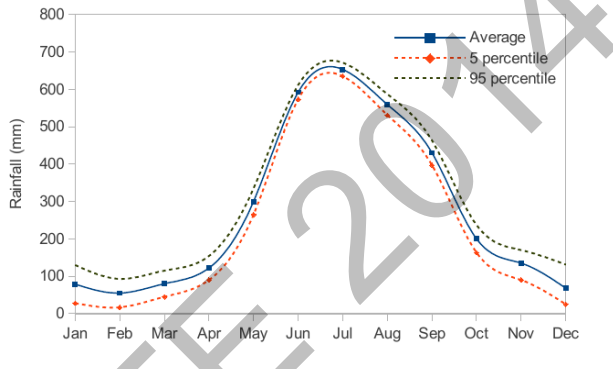
\includegraphics[width=0.5\columnwidth]{figs/q10.png}
\caption*{}
\label{fig:Q.10}
\end{figure}
\begin{enumerate}
\item On average, it rains more in July than in December
\item Every year, the amount of rainfall in August is more than that in January
\item July rainfall can be estimated with better confidence than February rainfall
\item In August, there is at least 500 mm of rainfall
\end{enumerate}

\hfill{\brak{\text{GATE AR 2014}}}
\begin{enumerate}
\item (i) and (ii)
\item (i) and (iii)
\item (ii) and (iii)
\item (iii) and (iv)
\end{enumerate}
\end{enumerate}

\section*{END OF THE QUESTION PAPER}

\section*{Q. 1 – Q. 25 carry one mark each.}

\begin{enumerate}

\item Toothling is a construction technique used in

\hfill{\brak{\text{GATE AR 2014}}}
\begin{enumerate}
\item Wood construction
\item Steel construction
\item Reinforced cement concrete construction
\item Brick masonry
\end{enumerate}

\item ‘Skeleton and Skin’ concept in building design and construction evolved during the

\hfill{\brak{\text{GATE AR 2014}}}
\begin{enumerate}
\item Roman period
\item Renaissance period
\item Gothic period
\item Greek period
\end{enumerate}

\item As per the IRC standards, the minimum width (in m) of a two lane urban carriageway without a raised kerb is

\hfill{\brak{\text{GATE AR 2014}}}
\begin{enumerate}
\item 6.0
\item 6.5
\item 7.0
\item 8.0
\end{enumerate}

\item Pritzker Architecture Prize 2013 has been awarded to
\begin{enumerate}
\item Mario Botta
\item Toyo Ito
\item Rem Koolhaas
\item Arata Isozaki
\end{enumerate}

\item Hip roof is formed by surfaces sloping in

\hfill{\brak{\text{GATE AR 2014}}}
\begin{enumerate}
\item One direction
\item Two directions
\item Three directions
\item Four directions
\end{enumerate}

\item Hiroshima Peace Memorial Museum in Japan has been designed by
\begin{enumerate}
\item Kenzo Tange
\item Kisho Kurokawa
\item Tadao Ando
\item I M Pei
\end{enumerate}

\item In AutoCAD, the maximum number of points which can be snapped in a circle using OSNAP command is

\hfill{\brak{\text{GATE AR 2014}}}
\begin{enumerate}
\item 1
\item 3
\item 4
\item 5
\end{enumerate}

\item Development authorities in India are established under the provision of

\hfill{\brak{\text{GATE AR 2014}}}
\begin{enumerate}
\item Municipal Act
\item $74^{th}$ Constitutional Amendment Act
\item Town and Country Planning Act
\item Land Acquisition Act
\end{enumerate}

\item In escalators, the angle of inclination with the horizontal plane should be in the range of

\hfill{\brak{\text{GATE AR 2014}}}
\begin{enumerate}
\item $10^\circ-20^\circ$
\item $20^\circ-30^\circ$
\item $30^\circ-35^\circ$
\item $35^\circ-45^\circ$
\end{enumerate}

\item As per the Census of India 2011, ‘Metropolitan Urban Agglomeration’ is a contiguous spread of several urban settlements where the minimum population size $\brak{\text{in Lakh}}$ is

\hfill{\brak{\text{GATE AR 2014}}}
\begin{enumerate}
\item One
\item Five
\item Ten
\item Fifty
\end{enumerate}

\item BEES is an acronym for

\hfill{\brak{\text{GATE AR 2014}}}
\begin{enumerate}
\item Building for Environmental and Economic Sustainability
\item Built Environment and Ecological Society
\item Building for Energy and Environment Sustainability
\item Built Environment and Engineering Services
\end{enumerate}

\item In a single-stack system of plumbing

\hfill{\brak{\text{GATE AR 2014}}}
\begin{enumerate}
\item All the appliances and traps are fully ventilated
\item Only WC branches are connected with anti-siphonage pipes
\item Anti-siphonage pipes are omitted
\item Only the stack is vented above the branch connection at each floor level
\end{enumerate}

\item The maximum bending moment $\brak{\text{kNm}}$ in a simply supported beam of 8 m span subjected to a uniformly distributed load of $20 kN/m$ $\brak{\text{inclusive of its self-weight}}$ over the entire span is

\hfill{\brak{\text{GATE AR 2014}}}
\begin{enumerate}
\item 40
\item 160
\item 240
\item 380
\end{enumerate}

\item Criteria for background noise (in NC) in hospitals and apartments is inclusive of its self-weight

\hfill{\brak{\text{GATE AR 2014}}}
\begin{enumerate}
\item $10-20$
\item $20-30$
\item $30-40$
\item $40-50$
\end{enumerate}

\item As per the National Building Code, the minimum width (in m) of a staircase flight in an educational building above 24 m height should be

\hfill{\brak{\text{GATE AR 2014}}}
\begin{enumerate}
\item 1.0
\item 1.5
\item 2.0
\item 2.5
\end{enumerate}

\item Among the following, the one that is NOT a land assembly technique is

\hfill{\brak{\text{GATE AR 2014}}}
\begin{enumerate}
\item Land Use Zoning
\item Accommodation Reservation
\item Town Planning Scheme
\item Transfer of Development Right
\end{enumerate}

\item The Grand Gallery in Egyptian Architecture is provided only at

\hfill{\brak{\text{GATE AR 2014}}}
\begin{enumerate}
\item Great Pyramid
\item Temple
\item Mastaba
\item Bent Pyramid
\end{enumerate}

\item In the Taipei 101 building, the steel sphere as TMD $\brak{\text{Tuned Mass Damper}}$ is suspended to reduce horizontal sway due to

\hfill{\brak{\text{GATE AR 2014}}}
\begin{enumerate}
\item Settlement \& Wind Load
\item Wind \& Geothermal Load
\item Seismic \& Geothermal Load
\item Seismic \& Wind Load
\end{enumerate}

\item ‘Finger Plan’ concept of urban planning was initially adopted in

\hfill{\brak{\text{GATE AR 2014}}}
\begin{enumerate}
\item Canberra
\item Paris
\item Copenhagen
\item Tokyo
\end{enumerate}

\item The most important property of concrete in its fresh state is

\hfill{\brak{\text{GATE AR 2014}}}
\begin{enumerate}
\item Compressive strength
\item Tensile strength
\item Elastic modulus
\item Workability
\end{enumerate}

\item An element constructed at intervals along the length of a wall to stabilize it against overturning is

\hfill{\brak{\text{GATE AR 2014}}}
\begin{enumerate}
\item Barrel Vault
\item Pilaster
\item Squinch Arch
\item Buttress
\end{enumerate}

\item Landscape design of Shakti Sthal, the ‘Samadhi’ of late Prime Minister Smt. Indira Gandhi, was done by architect

\hfill{\brak{\text{GATE AR 2014}}}
\begin{enumerate}
\item Ram Sharma
\item Mohammad Shaheer
\item Ravindra Bhan
\item Raj Rewal
\end{enumerate}

\item Horizontally Wedge-shaped Treads in stairways are termed as

\hfill{\brak{\text{GATE AR 2014}}}
\begin{enumerate}
\item Stringers
\item Winders
\item Scotia
\item Newel
\end{enumerate}

\item The sequence of development in a Site-and-Services scheme is

\hfill{\brak{\text{GATE AR 2014}}}
\begin{enumerate}
\item Land -- Service -- House -- Occupant
\item Occupant -- Land -- House -- Service
\item Occupant -- Land -- Service -- House
\item Land -- Occupant -- House -- Service
\end{enumerate}

\item Which of the following is NOT a classical spatial theory of land use planning?

\hfill{\brak{\text{GATE AR 2014}}}
\begin{enumerate}
\item Concentric Zone theory
\item Multiple Nuclei Theory
\item Centripetal Theory
\item Sector Theory
\end{enumerate}

\section*{Q. 26 – Q. 55 carry two marks each.}

\item A housing project is proposed to be designed in a plot of 2 hectare. Maximum permissible FAR is 2. The share of the numbers of dwelling units (DU) for MIG, LIG and EWS is 1:2:3 having sizes of 55, 35 and 25 sq.m respectively. The maximum number of DU which can be accommodated in the plot is \underline{\hspace{2cm}}

\item Arrange the following in ascending order of width

P. Collector Street\\
Q. Arterial Road\\
R. Local Street\\
S. Sub-Arterial Road

\hfill{\brak{\text{GATE AR 2014}}}
\begin{enumerate}
\item P, Q, S, R
\item R, P, S, Q
\item Q, S, R, P
\item Q, S, P, R
\end{enumerate}

\item Out of the following, the maximum points in the LEED (New construction) rating system can be earned through

\hfill{\brak{\text{GATE AR 2014}}}
\begin{enumerate}
\item Sustainable Sites
\item Water Efficiency
\item Materials and Resources
\item Energy and Atmosphere
\end{enumerate}

\item Which of the following is NOT a mechanism of bond resistance in reinforced concrete?

\hfill{\brak{\text{GATE AR 2014}}}
\begin{enumerate}
\item Chemical adhesion
\item Friction
\item Mechanical interlock
\item Aggregate interlock
\end{enumerate}

\item A neighborhood has 250 units of 80 sq.m each and 200 units of 100 sq.m each. If the mandatory parking requirement is one per 100 sq.m of built space then, the total area (sq.m) required for parking considering 30 percent additional area for circulation is \underline{\hspace{2cm}}

\hfill{\brak{\text{GATE AR 2014}}}

\item A brick wall 19 cm thick has a thermal conductivity 0.811 W/m$^\circ$C. The outside and inside surface conductance of the wall are 16 W/m$^2$$^\circ$C and 8 W/m$^2$$^\circ$C respectively, then the U-value of the wall in W/m$^2$$^\circ$C is \underline{\hspace{2cm}}

\item Match the contemporary buildings in Group I with their architects in Group II

\begin{table}[H]
\centering
\begin{tabular}{c|c}
Group I & Group II \\
\hline
Vitra Design Museum, Basel & Adrian Smith \\
Turning Torso, Malmö & Jean Nouvel \\
Burj Khalifa, Dubai & Herzog de Meuron \\
Tate Modern, London & Santiago Calatrava \\
 & Frank O Gehry \\
\end{tabular}
\caption*{}
\label{tab:Q.32}
\end{table}

\hfill{\brak{\text{GATE AR 2014}}}
\begin{enumerate}
\item P-3, Q-4, R-2, S-5
\item P-5, Q-4, R-1, S-3
\item P-5, Q-3, R-2, S-1
\item P-5, Q-3, R-1, S-2
\end{enumerate}

\item From the following cost components of a building construction project which is not a direct cost combination?

P. Labour cost \\
Q. Equipment cost \\
R. Material cost \\
S. Establishment cost \\
T. Supervision cost

\hfill{\brak{\text{GATE AR 2014}}}
\begin{enumerate}
\item P and Q
\item Q and R
\item P and R
\item S and T
\end{enumerate}

\item A house located in Delhi has 111 m$^2$ of flat terrace area (runoff coefficient = 0.85) and 55 m$^2$ of ground area covered with grass (runoff coefficient = 0.15). If annual average rainfall is 611.8 mm, then rain water harvesting potential (L/year) from runoff will be \underline{\hspace{2cm}}

\hfill{\brak{\text{GATE AR 2014}}}

\item Match the elements in Group I with the structures in Group II

\begin{table}[H]
\centering
\begin{tabular}{c|c}
Group I & Group II \\
\hline
Harmika & Dilwara Temple, Mount Abu \\
Sixteen Vidyadevis & sun Temple, Modhera \\
Lat pillar & Stupa of sanchi \\
Urushringa & Lauriya, Nandangarh \\
 & Great Kailash Temple, Ellora \\
\end{tabular}
\caption*{}
\label{tab:Q.35}
\end{table}

\hfill{\brak{\text{GATE AR 2014}}}
\begin{enumerate}
\item P-5, Q-1, R-4, S-3
\item P-1, Q-2, R-4, S-3
\item P-3, Q-5, R-4, S-2
\item P-3, Q-1, R-4, S-2
\end{enumerate}

\item A site, based on percolation test, the allowable rate of treated sewage application was determined as 65 L/m$^2$/day. The effective depth (m) of a soak pit with a diameter of 2.5 m for the disposal of 1020 L/day of septic tank effluent is \underline{\hspace{2cm}}

\hfill{\brak{\text{GATE AR 2014}}}

\item Match the AutoCAD command in Group I with their functions in Group II

\begin{table}[H]
\centering
\begin{tabular}{c|c}
OOPS & Creates solid lines \\
\hline
RAY & Restores an erased drawing \\
\hline
TRACE & Manages customized user interface elements \\
\hline
CUI & Creates semi-infinite lines \\
\hline
 & Creates a five sided 3D solid with a sloped face tapering along the X axis \\
\end{tabular}
\caption*{}
\label{tab:Q.37}
\end{table}

\hfill{\brak{\text{GATE AR 2014}}}
\begin{enumerate}
\item P-1, Q-3, R-2, S-5
\item P-2, Q-4, R-1, S-3
\item P-2, Q-1, R-3, S-4
\item P-1, Q-2, R-3, S-4
\end{enumerate}

\item Match the bridges in Group I with their structure type in Group II

\begin{table}[H]
\centering
\begin{tabular}{c|c}
\textbf{Group I} & \textbf{Group II}\\
\hline
Harbour Bridge, Sydney & 1. Simply Supported \\
Golden Gate Bridge, San Francisco & 2. Cable Stayed \\
Howrah Bridge, Kolkata & 3. Arch \\
Millau Viaduct, Millau & 4. Suspension \\
 & 5. Cantilever \\
\end{tabular}
\caption*{}
\label{Q.38}
\end{table}

\hfill{\brak{\text{GATE AR 2014}}}
\begin{enumerate}
\item P-3, Q-4, R-5, S-2
\item P-2, Q-3, R-4, S-5
\item P-5, Q-1, R-4, S-3
\item P-1, Q-2, R-3, S-4
\end{enumerate}

\item The arithmetic average value of the sound absorption coefficient for a specific material and particular mounting condition for four frequencies is

\hfill{\brak{\text{GATE AR 2014}}}
\begin{enumerate}
\item Transmission coefficient
\item Noise reduction coefficient
\item Absorption coefficient
\item Reflection coefficient
\end{enumerate}

\item A single span simply supported reinforced concrete beam $\brak{\text{250 mm wide and 480 mm effective depth}}$ is subjected to a concentrated load of $120 kN$ at its mid-span. Neglecting self-weight of the beam, the nominal shear stress $\brak{\text{MPa}}$ at the support section is\underline{\hspace{3cm}}

\hfill{\brak{\text{GATE AR 2014}}}
    
\item The optimistic time, the pessimistic time and the most likely time of a job are 6, 13 and 8 days respectively. The variance for this job is \underline{\hspace{3cm}}

\hfill{\brak{\text{GATE AR 2014}}}

\item A refuse collection system consisting of two chutes is to be provided in a 20 storied residential building with 2 flats/floor $\brak{\text{average family size = 5}}$ and with each chute serving one flat on each floor. Average quantity of refuse and its density are 880 g/person/day and 240 kg/m$^3$ respectively. If the cleaning interval is two days, then the minimum size of the refuse container $\brak{\text{litre}}$ at the bottom of each chute is \underline{\hspace{3cm}}

\hfill{\brak{\text{GATE AR 2014}}}

\item Match the features in Group I with their architectural periods in Group II

\begin{table}[H]
\centering
\begin{tabular}{c|c}
Group I & Group II\\
\hline
Caryatids & Roman \\
Hypocaust & Gothic \\
Pylons & Greek \\
Lofty Pinnacles & Egyptian \\
 & Romanesque \\
\end{tabular}
\caption*{}
\label{Q.43}
\end{table}

\hfill{\brak{\text{GATE AR 2014}}}
\begin{enumerate}
\item P-1, Q-5, R-4, S-2
\item P-5, Q-1, R-3, S-2
\item P-3, Q-2, R-5, S-4
\item P-3, Q-1, R-4, S-2
\end{enumerate}

\item Match the following terminologies in Group I with their descriptions in Group II

\begin{table}[H]
\centering
\begin{tabular}{c|c}
Group I & Group II \\
\hline
Pruning & Useful in reproducing plants that would not breed true if propagated by seed \\
Topiary & A live bud from a desired plant inserted into a host plant \\
Grafting & Cutting of evergreen shrubs into abstract or geometric shapes \\
Budding & Trimming and cutting of lawns \\
 & Selective cutting of plant branches for better growth \\
\end{tabular}
\caption*{}
\label{Q.44}
\end{table}

\hfill{\brak{\text{GATE AR 2014}}}
\begin{enumerate}
\item P-5, Q-3, R-4, S-2 
\item P-2, Q-3, R-1, S-5
\item P-3, Q-4, R-1, S-2
\item P-5, Q-3, R-1, S-2
\end{enumerate}

\item In a dance hall the indoor and outdoor temperatures are 28$^\circ$C and 18$^\circ$C respectively. There is an internal heat gain of 5 kW and the specific heat of air $\brak{\text{on volume basis}}$ is $1300 J/m^3~^\circ$C, then the necessary cross sectional area $\brak{m^2}$ of a duct with an air velocity of 2 m/s required for cooling by ventilation is \underline{\hspace{4cm}}

\hfill{\brak{\text{GATE AR 2014}}}

\item Assuming full compaction, strength of concrete is inversely proportional to

\hfill{\brak{\text{GATE AR 2014}}}
\begin{enumerate}
\item Water - cement ratio
\item Water - sand ratio
\item Water - coarse aggregate ratio
\item Water - plasticiser ratio
\end{enumerate}

\item Match the terms in Group I with their examples in Group II

\begin{table}[H]
\centering
\begin{tabular}{c|c}
Group I & Group II \\
\hline
Incentive zoning & Boardwalk, Atlantic City \\
Universal design & Minneapolis, USA \\
Promenading & Broadway Theatre District, New York \\
Skyway system & Pruitt Igoe Housing, St. Louis, Missouri \\
 & Curitiba, Brazil \\
\end{tabular}
\caption*{}
\label{Q.47}
\end{table}

\hfill{\brak{\text{GATE AR 2014}}}
\begin{enumerate}
\item P-5, Q-3, R-2, S-1
\item P-4, Q-5, R-1, S-3
\item P-3, Q-5, R-4, S-2
\item P-3, Q-5, R-1, S-2
\end{enumerate}

\item If yield stress of steel is $415 MPa$, then strain in tensile reinforcement at the limit state of collapse shall be at least \underline{\hspace{2.5cm}}. For steel, the Young's Modulus, $E = 2 \times 10^5 MPa$.

\hfill{\brak{\text{GATE AR 2014}}}

\item Match the books in Group I with their authors in Group II

\begin{table}[H]
\centering
\begin{tabular}{c|c}
Group I & Group II \\
\hline
Architecture now! & Ian Mc Harg \\
Intentions in architecture & Robert Venturi \\
Design with Nature & Christopher Alaxander \\
Complexity & Contradictions in Architecture \& Philip Jodidio \\
 & Christian Norberg Schulz \\
\end{tabular}
\caption*{}
\label{tab:Q.49}
\end{table}

\hfill{\brak{\text{GATE AR 2014}}}
\begin{enumerate}
\item P-2, Q-3, R-4, S-1
\item P-4, Q-5, R-1, S-2
\item P-3, Q-1, R-5, S-2
\item P-3, Q-1, R-4, S-2
\end{enumerate}

\item Match the common names of the trees in Group I with their botanical names in Group II

\begin{table}[H]
\centering
\begin{tabular}{c|c}
Group I & Group II \\
\hline
Gulmohar & Dalbergia Sissoo \\
Palas & Ficus Benghalensis \\
Indian Mahogany & Delonix Regia \\
Banyan & Toona Ciliata \\
 & Butea Monosperma \\
 \end{tabular}
 \caption*{}
 \label{Q.50}
 \end{table}

\hfill{\brak{\text{GATE AR 2014}}}
\begin{enumerate}
\item P-5, Q-3, R-4, S-2
\item P-4, Q-5, R-2, S-1
\item P-3, Q-1, R-5, S-2
\item P-3, Q-1, R-4, S-2
\end{enumerate}

\item A room of internal dimension $4m \times 9m \times 3.5m \brak{LxBxH}$ has $20 cm$ thick walls and two doors of size $1m \times 2m$. The required area for Damp Proof Course $\brak{sq.m}$ is \underline{\hspace{3cm}}.

\hfill{\brak{\text{GATE AR 2014}}}

\item A load of $30 kN$ is applied vertically downward at the free end of a cantilever of span $5 m$. If the elastic modulus of the cantilever is $30 GPa$ and the section has a width of 0.3 m and a depth of 0.6 m, then, the elastic deflection $\brak{\text{in mm}}$ is \underline{\hspace{3cm}}.

\hfill{\brak{\text{GATE AR 2014}}}

\item Associate the plans in Group I with the options in Group II

\begin{table}[H]
\centering
\begin{tabular}{c|c}
Group I & Group II \\
\hline
City Development Plan & PMGSY \\
Slum Free City Plan & JNNURM \\
Transport Network Plan & RAY \\
Disaster Management Plan & NDMA \\
 & RSVY \\
\end{tabular}
\caption*{}
\label{Q.53}
\end{table}

\hfill{\brak{\text{GATE AR 2014}}}
\begin{enumerate}
\item P-2, Q-3, R-1, S-4
\item P-2, Q-1, R-5, S-4
\item P-1, Q-3, R-2, S-5
\item P-3, Q-2, R-1, S-4
\end{enumerate}

\item The capacity of a hall is 600 persons and its volume is $3000 cu.m$. If an optimum reverberation time of 1.0 second is to be achieved then the required total absorption $\brak{m^2 sabine}$ is \underline{\hspace{2cm}}.

\hfill{\brak{\text{GATE AR 2014}}}

\item A solid straight steel rod of diameter $100 mm$ is bent in single curvature into a circular arc by a moment of $50 kNm$ applied at its ends. If elastic modulus, E, for steel is $2 \times 105 MPa$, the radius of curvature $\brak{mm}$ of the arc assuming $\pi=3.14$ is \underline{\hspace{2cm}}.

\hfill{\brak{\text{GATE AR 2014}}}

\section*{END OF THE QUESTION PAPER}
\end{enumerate}

\end{document}